\documentclass[a4paper,english]{lipics-v2019}

\usepackage[all]{xy}
\usepackage{amsmath}
\usepackage{amssymb}
\usepackage{amsthm}
%\usepackage[notref,notcite]{showkeys}
\usepackage{color}
\usepackage{graphicx}
\usepackage{xspace}
\usepackage{enumerate}
\usepackage{mathtools}
\usepackage{tikz}%rysowanie macierzy
\usetikzlibrary{matrix,positioning}

\newtheorem{Par}[theorem]{\S}
\newtheorem{Quest}[theorem]{Q}
\newtheorem{todo}[theorem]{To do}

\newtheorem{fact}[theorem]{Fact}



\newcommand{\clone}{\mathsf C}
\newcommand{\clonereg}{\mathsf C^{\mathrm{reg}}}
\newcommand{\rank}[1]{\mathrm{rank}(#1)}
\newcommand{\diva}{{\sc{(da)}}}
\newcommand{\homf}{{\sc{(hf)}}}
\newcommand{\fing}{{\sc{(fg)}}}
\newcommand{\eqdef}{\stackrel{\text{\tiny def}}=}
\newcommand{\trees}{{\mathsf{trees}}}
\newcommand{\terms}[1]{{\mathsf T}\!_{#1}}
\newcommand{\powerset}{{\mathsf P}}
\newcommand{\muddles}{{\mathsf M}}
\newcommand{\unit}{\mathsf{unit}}
\newcommand{\flatt}{\mathsf{flat}}
\newcommand{\aalg}{\ensuremath{\mathbf{A}}\xspace}
\newcommand{\balg}{\ensuremath{\mathbf{B}}\xspace}
\newcommand{\Nat}{\mathbb N}
\newcommand{\hsp}{{\sc hsp \xspace}}
\newcommand{\mso}{{\sc mso}\xspace}
\newcommand{\msoone}{{\sc mso$_1$ \xspace}}
\newcommand{\msotwo}{{\sc mso$_2$ \xspace}}

\newcommand{\hs}{{\sc hs \xspace}}
\newcommand{\aut}{\mathcal A}
\newcommand{\nodes}{\mathsf{nodes}}
\newcommand{\set}[1]{\{#1\}}
\newcommand{\dom}{\mathsf{dom}}
%\newcommand{\ker}{\mathsf{ker}}
\newcommand{\game}{\mathsf G}
\newcommand{\mult}{\mathsf{mult}}
\newcommand{\parfun}{\rightharpoonup}
\newcommand{\monad}{\mathsf M}
\newcommand{\facto}{\mathsf F}
\newcommand{\poly}[2]{\mathsf{pol}_{#1}#2}

%
%%Janusz%%
\newcommand{\ens}[1]{{\ensuremath{#1}}\xspace}
%Strzałki
\newcommand{\ra}{\rightarrow}
\newcommand{\xra}[1]{\xrightarrow{#1}}
\newcommand{\Z}{\ensuremath{\mathbb{Z}}\xspace}
\DeclareMathOperator{\join}{fuse}
\DeclareMathOperator{\forget}{forget}
\DeclareMathOperator{\sources}{sources}
\DeclareMathOperator{\cyclic}{cycle}
\DeclareMathOperator{\charact}{char}%komenda \char jest już defined
\newcommand{\allv}[1]{\ensuremath{\sources(#1) \cup \{\bullet\}}\xspace} %"allv = all vertices", czyli source'y plus \bullet
\newcommand{\Registers}{\ensuremath{\mathcal{R}}\xspace}
\newcommand{\enum}[3]{#1_{#2}, \ldots, #1_{#3}}
\newcommand{\iffdef}{\stackrel{def}{\Leftrightarrow}}
\newcommand{\N}{\ens{\mathbb{N}}}
\newcommand{\Q}{\ens{\mathbb{Q}}}
\newcommand{\Cc}{\ensuremath{\mathcal{C}}\xspace}
\def\sizemacierzy{0.4cm}
\def\GaSize{\large}
\def\ZeroSize{\Large}
\def\GprimSize{\Large}
\def\HprimSize{\LARGE}
\newlength{\picPrzesuniecie}
\setlength{\picPrzesuniecie}{4.5cm}
\def\skalamatadjacency{0.8}
\def\skalamacierzy{1}
\newcommand{\primecofact}[2]{\overline{#1}^{#2}}%definicja phi dla wielomianu charakterystycznego -- pierwszy komponent, argumenty #1 = graf, #2 = nazwa source'a względem którego sklejamy
\newcommand{\rest}[2]{\widetilde{#1}^{#2}}%definicja phi dla wielomianu charakterystycznego -- drugi komponent, argumenty #1 = graf, #2 = nazwa source'a względem którego sklejamy
\newcommand{\algcyclic}{\ensuremath{\mathbf{C}}\xspace}
\newcommand{\algebradefinition}[2]%argumenty to: Uniwersum i Operacje
{
	{
		\begin{description}
			\item[Domain:] \hfill \\ #1
			\item[Operations:] \hfill \\ #2
		\end{description}
	}
} 
\newcommand{\op}{\ensuremath{\tau}\xspace}
%register transducers
\def\valu{\mathbf{v}}
\DeclareMathOperator{\out}{output}
\newcommand{\qinit}{\ensuremath{q_{init}}\xspace}
\newcommand{\initval}{\ensuremath{{\mathbf{t}_0}}\xspace}

%Hilbert Method
%
\newcommand{\simby}{\preceq_{pol}}
%\newcommand{\Registers}{\ens{\mathcal{R}}}
\newcommand{\Transitions}{\ens{\Delta}}
\newcommand{\bt}{\ens{\mathbf{t}}}
\newcommand{\InputAlphabet}{\ens{\Sigma}}
\newcommand{\Input}{\ens{\Sigma^*}}
\newcommand{\cl}[1]{\ens{\overline{#1}}}
\newcommand{\COSq}[1]{\ens{(#1_q)_{q \in Q}}}
\newcommand{\Fq}{\COSq{F}}
\newcommand{\Iq}{\COSq{I}}
\newcommand{\Xq}{\COSq{X}}
\DeclareMathOperator{\II}{\mathcal{I}}
\DeclareMathOperator{\VV}{\mathcal{V}}
%%Janusz-koniec
%
\newcounter{ourexamplecounter}
\newenvironment{example}{
\medskip

\refstepcounter{ourexamplecounter}
\smallskip\noindent{\textbf{{Example \arabic{ourexamplecounter}. }}}}{
$\Box$ \smallskip 
}

\newcounter{runningcounter}
\newenvironment{running}{
\medskip

\refstepcounter{runningcounter}
\smallskip\noindent{\textbf{{Running Example \arabic{runningcounter}. }}}}{
$\Box$ \smallskip 
}




\newcommand{\mypic}[1]{
	\begin{center}
		\includegraphics[page=#1,scale=0.4]{pics}
	\end{center}
}

\newcommand{\treewidthtotreewidth}[2]{treewidth$_{\leqslant #1}$-to-treewidth$_{\leqslant #2}$}

\newcommand{\treetotreewidth}[1]{tree-to-treewidth$_{< #1}$\xspace}

\newcommand{\homset}{\mathrm
{Hom}}

\newcommand{\powerseries}[1]{#1 [\![x]\!]}
\newcommand{\natx}{\Nat_{0}[\![x]\!]}
% \newcommand{\powerseries}[1]{\mathbb Q [\![#1]\!]}

\newcommand{\Ring}{\mathbb K}
\newcommand{\Rat}{\mathbb Q}
\newcommand{\Int}{\mathbb Z}
\newcommand{\Real}{\mathbb R}
% \newcommand{\Nat}{\mathbb N}


\newcommand{\smallparagraph}[1]{\smallskip \noindent {\bf #1. }}

\newcommand{\Rr}{{\mathcal R}}
\newcommand{\Ss}{{\mathcal S}}
\newcommand{\Tt}{{\mathcal T}}
\newcommand{\Ff}{{\mathcal F}}
\newcommand{\myunderbrace}[2]{\underbrace{#1}_{\mathclap{\text{#2}}}}
\newcommand{\myoverbrace}[2]{\overbrace{#1}^{\mathclap{\text{#2}}}}

\newcommand{\Aa}{{\ens{\mathcal A}}}
\newcommand{\Bb}{{\mathcal B}}

\newcommand{\decisionproblem}[3]
{
	\begin{description}
		\item[Name:] #1
		\item[Instance:]  #2
		\item[Question:] #3 
	\end{description}
}
\DeclareMathOperator{\eqzeroinalgb}{\ensuremath{
		%p_{((-) =_B)}
		p_{0_B}
	}}
\newcommand{\Zrat}{\ens{\Z^{rat}[\![x]\!]}}

\title{Some remarks on deciding equivalence for graph-to-graph transducers}
\author{Miko\l aj Boja\' nczyk}{Institute of Informatics,\\ University of
Warsaw, Poland}{bojan@mimuw.edu.pl}{}{}

\author{Janusz Schmude}{Institute of Informatics,\\ University of
Warsaw, Poland}{jschmude@mimuw.edu.pl}{}{}
\begin{document}

\authorrunning{M. Boja\'nczyk and J. Schmude}%TODO mandatory. First: Use abbreviated first/middle names. Second (only in severe cases): Use first author plus 'et al.'

\Copyright{Miko{\l}aj Boja\'nczyk and Janusz Schmude}%TODO mandatory, please use full first names. LIPIcs license is "CC-BY";  http://creativecommons.org/licenses/by/3.0/

\ccsdesc[100]{Theory of computation~Formal languages and automata}%TODO mandatory: Please choose ACM 2012 classifications from https://dl.acm.org/ccs/ccs_flat.cfm 

\maketitle

\begin{abstract}
    We  study the following decision problem: given two \mso transductions that input and output graphs bounded treewidth, decide if they are equivalent, i.e.~isomorphic inputs give isomorphic outputs. We do not know  if this problem is decidable, but  we  propose an approach to deciding the problem which uses algebra. We  show how the approach can be successful for a variant of the problem, where instead of isomorphism on output graphs, we consider certain relaxations of isomorphism.
\end{abstract}
\section{Introduction}


% (ideally, graph isomorphism) for every input graph, the output graphs produced by the two transductions are isomorphic.  we state a problem and propose a solution strategy. The problem is deciding  equivalence for graph-to-graph transductions, for graphs of bounded treewidth. The solution strategy is to model graphs as algebraic objects (polynomials, or rational power series) and to use algorithms from algebra (Hilbert's Basis Theorem, or Gr\"obner bases) to decide equivalence. 



% \begin{itemize}
%     \item {\bf Parameter.} A number $k \in \set{1,2,\ldots}$ and an equivalence relation $\sim$ on graphs. 
%     \item {\bf Input.}  Two mso transductions 
%     \begin{align*}
%         \xymatrix@C=3cm{
%     \text{graphs of treewidth $k$} 
%     \ar[r]^{f_1,f_2} &
%      \text{graphs of treewidth $k$}}
%     \end{align*}
%     \item {\bf Output.} Is $f_1$ equivalent to $f_2$ modulo $\sim$, i.e.~is it the case that
%     \begin{align*}
%     f_1(G) \sim f_2(G) \qquad \text{for every graph $G$ of treewidth $\le k$.}
%     \end{align*}
% \end{itemize}

% Our long term goal is to find out if the problem above is decidable or not  when  $\sim$ being graph isomorphism, and $k$ is arbitrary. In this paper, we show decidability for two special cases:
% \begin{itemize}
%     \item $\sim$ is isomorphism and $k=1$;
%     \item $\sim$ is a .. and $k$ is arbitrary.
% \end{itemize}


% \begin{lemma}
%     Given  mso transductions 
%     \begin{align*}
%         \xymatrix@C=3cm{
%     \text{graphs of treewidth $\le k$} 
%     \ar[r]^{f_1,f_2} &
%      \text{graphs of treewidth $\le k$}}
%     \end{align*}
%     one can compute mso transductions
%     \begin{align*}
%         \xymatrix@C=3cm{
%     \text{trees} 
%     \ar[r]^{g_1,g_2} &
%      \text{graphs of treewidth $\le k$}}
%     \end{align*}
% \end{lemma}
\section{Graphs, treewidth, and logic on graphs}
The graphs in this paper are finite and undirected, without  parallel edges. 

\subsection{Treewidth}
\label{sec:treewidth-definition}
The kind of problems studied in this paper (equivalence for \mso transductions) become immediately undecidable for graphs of unbounded treewidth. Therefore, we  only consider classes of graphs of bounded treewidth.  To define treewidth, we use Courcelle's  approach via universal algebra. (Later on in the paper, we also use algebra in the classical sense: rings, fields, polynomials, etc.)


\smallparagraph{Algebras, terms and polynomials} We begin by introducing some terminology from universal algebra. By an \emph{algebra}, we mean a set equipped with some  operations, e.g.~the ring of integers $(\Int, + , \times, 0, 1)$ or the free monoid $(\Sigma^*, \cdot, \varepsilon)$. We write $\aalg, \balg, \ldots$ for algebras. By abuse of notation, we write $a \in \aalg$ if $a$ belongs to the underlying set in the algebra $\aalg$. 
        For $k \in \set{0,1,\ldots}$, define a \emph{$k$-ary term operation in an algebra $\aalg$} to be  any operation of type $\aalg^k \to \aalg$ that arises from a term constructed using $k$ variables (representing inputs of the operation) and operations of the algebra. For example, 
        \begin{align*}
        (x,y) \qquad \mapsto \qquad xyxxxy
        \end{align*}
        is a binary term operation in the free monoid. 
        A \emph{$k$-ary polynomial operation} is defined the same way, except that the term can also use all elements of the algebra as constants.  For example, 
        \begin{align*}
        (x,y) \qquad \mapsto \qquad  xyabaxyxa
        \end{align*}
        is a binary polynomial in the free monoid with $a,b \in \Sigma$. Here is another example, which explains the terminology: if  the algebra $\aalg$ is 
        $
        (\Real, + , \times, 0 ,1)
        $
        then the $k$-ary term operations are the same as polynomials with $k$ variables with coefficients in $\set{0,1,\ldots}$, while the $k$-ary polynomial operations are the same as (general) polynomials with $k$ variables.

        
\smallparagraph{The algebra of $k$-sourced graphs} To define treewidth, we consider graphs with distinguished vertices and equip them with an algebraic structure. 
    Let $k \in \set{1,2,\ldots}$. Define a $k$-sourced graph to be a  graph together with a $k$-tuple of pairwise distinct vertices called \emph{sources}. We allow sources to be undefined; in particular when all sources are undefined then we get a graph. Here is a 
    picture of a 3-sourced graph, where sources 1 and 3 are defined, but source 2 is undefined:
    \mypic{2}
    We view  $k$-sourced graphs as an algebra, in the following sense.



    
    \begin{definition}
        [Algebra of $k$-sourced graphs] Let $k \in \set{1,2,\ldots}$. The \emph{algebra of $k$-sourced graphs} has as its underlying set the  $k$-sourced graphs, equipped with the following operations:
            \begin{itemize}
                \item {\bf Constants.} Every $k$-sourced graph with at most $k+1$ vertices is a constant.
                \item {\bf Forget.} For every $i \in \set{1,\ldots,k}$ there is a unary operation, which inputs a $k$-sourced graph and outputs the same $k$-sourced graph, except that the $i$-th source is undefined. 
                \item {\bf Fuse.} There is one binary operation, called \emph{fusion}, which inputs two $k$-sourced graphs, and output their disjoint union, with same-numbered sources being identified, as explained in the following picture:
                \mypic{1}
            \end{itemize}
        \end{definition}
    
  

    \begin{lemma}
        A graph has treewidth $\le k$, in the sense of Robertson and Seymour,  if and only if it is the value of an arity zero term in the algebra of $k$-sourced graphs.
    \end{lemma}
    % \begin{definition}[Treewidth]
    %     For $k \in \set{1,2,\ldots}$, we say that a  graph has treewidth  $\le k$ if it can be produced using the operations of the algebra of $(k+1)$-sourced graphs.
    % \end{definition}

    % The definition above coincides with the original definition of Robertson and Seymour, which uses tree decompositions with bags of vertices~\cite[Proposition 1.19]{courcelle1991}. 

    \subsection{Monadic second-order logic}
    We will use logic, especially monadic second-order logic, to define properties of graphs and transformations on graphs. 

    \smallparagraph{Logical terminology}
    We use the name  \emph{vocabulary} for a set of relation names, each one with an associated arity. A \emph{model over a vocabulary $\tau$} consists of a universe together with an interpretation of the relations names in the vocabulary $\tau$, which maps each relation name to a relation over the universe of same arity. To define properties of such models, we use mainly monadic second-order logic \mso, which  is the extension of first-order logic that allows quantification over sets of elements (but not sets of pairs, or triples, etc.). We assume that the reader is familiar with \mso, for an introduction see~\cite[Section 2]{Thomas97}.
     
     
      To define properties of graphs in \mso, we represent a graph as models. There are two representations, called  \msoone and \msotwo following 
 Courcelle~\cite[Definition 1.7]{courcelleVI}. In the \msoone model, the  universe is the vertices and there is a binary relation for the edges (the binary relation is symmetric, because graphs are undirected). In the \msotwo model, the universe is the disjoint union of vertices and edges, and there is a binary  \emph{incidence relation} that consists of pairs $(v,e)$ such that vertex $v$ participates in edge $e$. 
In this paper, we use the \msotwo model. More properties of graphs can be expressed in \mso with this representation, e.g.~existence of a Hamiltonian cycle can be expressed using the \msotwo representation but not with the \msoone representation~\cite[p.~118]{courcelleVI}. However, for graphs of bounded treewidth, \msoone and \msotwo have the same expressive power~\cite{}. 

\smallparagraph{Transductions}  The central topic of this paper is \mso transductions, which are graph transformations definable in \mso. In principle, the transductions are nondeterministic -- i.e.~they represent binary relations and not functions -- but we will show that the case of functions is general for the equivalence problems that we consider.

% \begin{definition}\label{def:graph-to-graph-mso}
%     The syntax of a graph-to-graph \mso transduction consists of:
%         \begin{enumerate}
%             \item a finite set of colours $C$;
%             \item a copying constant $k \in \set{1,2,\ldots}$;
%             \item \label{msotrans:formulas} two \mso formulas -- a universe formula with one free variable, and an incidence formula with two free variables --  over the following relational vocabulary
%             \begin{align*}
%             \underbrace{\mathrm{incident}(x_1,x_2)}_{\txt{arity 2}}  \qquad
%             \underbrace{\mathrm{copy}(x_1,\ldots,x_k)}_{\txt{arity $k$}}  \qquad 
%             \underbrace{\mathrm{colour}_c(x)\ \text{for $c \in C$}}_{\txt{arity 1}}.
%             \end{align*}
%         \end{enumerate}
% \end{definition}
% The semantics of an \mso transdution is a binary relation on graphs, which is defined as follows. The idea is that we take an input graph, colour its vertices with colours from $C$, copy each vertex $k$ times, and then use the formulas from item~\ref{msotrans:formulas} to define a new graph structure. Since there are many ways of choosing the colouring, the same input graph might lead to several different output graphs. A more formal definition is given below.

%  Consider an input graph $G$ together with a colouring $\lambda$ of the vertices by colours from $C$.  Consider a relational structure   which is defined as follows. The universe is pairs $(x,i)$ such that $x$ is either a vertex or edge in $G$, and $i \in \set{1,\ldots,k}$. The   vocabulary is the same as in item~\ref{msotrans:formulas} of Definition~\ref{def:graph-to-graph-mso}, with the relations from the vocabulary interpreted as follows:
% \begin{align*}
% \mathrm{incident} = & \set{((v,i),(e,i)) : (v,e) \text{ is incident in $G$ and $i \in \set{1,\ldots,k}$}}\\
% \mathrm{copy} = & \set{((v,1),\ldots,(v,k)) : \text{$v$ is a vertex of $G$ and $i \in \set{1,\ldots,k}$}} \\
% \mathrm{color}_c = & \set{(v,i) : \text{$v$ is a vertex of $G$ with colour $c$ and $i \in \set{1,\ldots,k}$}}
% \end{align*}
% Define  $G_\lambda$ to be the relational structure,   with one binary incidence relation, which arises from the above relational structure by restricting the universe to those elements which satisfy the universe formula, and defining the incidence relation to be those pairs which satisfy the incidence formula.  The semantics of the \mso interpretation is defined to be 
% \begin{align*}
% \set{(G,H) : \text{the \msotwo encoding of $H$ is isomorphic to $G_\lambda$, for some $\lambda$}}
% \end{align*}
 A transduction, with input vocabulary $\tau$ and output vocabulary $\sigma$ is a set of pairs 
\begin{align*}
    (\myunderbrace{\text{model over $\tau$}}{input model}, \ 
    \myunderbrace{\text{model over $\sigma$}}{output model}),
\end{align*}
which is isomorphism invariant, in the sense that membership in the transduction is not affected by changing a model -- on either the input or output coordinate -- to an isomorphic one. The central topic of this paper is transductions that can be defined using \mso, as described in the following definition, whose phrasing is based on~\cite[p.~9--10]{bojanczykOptimizingTreeDecompositions2017a}. 

\begin{definition}[\mso transduction]\label{def:mso-transduction}
    An \mso transduction is any transduction that can be obtained by composing a finite number of transductions of the following kinds.
Kind 1 is a partial function, kinds 2, 3, 4 are functions, and kind 5 is a relation.
\begin{enumerate}
	\item {\bf Filtering.} For every \mso sentence $\varphi$ over the input vocabulary there is a transduction that filters out models where $\varphi$ is violated. Formally, the transduction is the partial identity -- with input and output vocabularies being equal --  whose domain consists of the models that satisfy the sentence. 
	\item {\bf Universe restriction.} For every \mso formula $\varphi(x)$ over the input vocabulary with one free first-order variable, there is a transduction, which restricts the universe of the input model to those elements that satisfy $\varphi$. The input and output vocabularies are the same, the interpretation of each relation in the output model is defined as the restriction of its interpretation 
	in the input model to tuples of elements that remain in the universe.
	\item {\bfseries{\scshape{Mso}} interpretation.} This kind of transduction changes the vocabulary of the model while keeping the universe intact. To specify an \mso interpretation, for for every relation name $R$ of the output vocabulary, one gives an \mso formula $\varphi_R(x_1,\ldots,x_k)$ over the input vocabulary which has as many free first-order variables as the arity of $R$. The output model is obtained from the input model by keeping the same universe, and interpreting each relation $R$ of the output vocabulary as the set of tuples  satisfying $\varphi_R$.
	\item {\bf Copying.} For  $k \in \set{1,2,\ldots}$, define $k$-copying to be the transduction which inputs a model and outputs a model consisting of $k$ disjoint copies of the input, with an additional relation that ties the copies together. Formally, the output universe consists of $k$ copies of the input universe.
	The output vocabulary is the input vocabulary enriched with a binary predicate $\mathsf{copy}$ which selects pairs which originate from the same element, and unary predicates $\mathsf{layer}_1,\mathsf{layer}_2,\ldots,\mathsf{layer}_k$ which select elements belonging to the first, second, etc. copies of the universe.
	In the output model, a relation name $R$ of the input vocabulary is interpreted as the set of all those tuples over the output model, which are in the same layer, and  where the original elements of the copies were in relation $R$
	in the input model.
	\item {\bf Colouring.} Colouring adds  a new unary predicate to the input model, and interprets it nondeterministically. Formally, the universe as well as the interpretations of all relation names of the input vocabulary stay intact,
	but the output vocabulary has one more unary predicate. For every possible interpretation of this unary predicate, there is a different output with this interpretation implemented.
\end{enumerate}
\end{definition}

\smallparagraph{The equivalence problem}  Define a \emph{graph-to-graph \mso transduction} to be an \mso transduction, where the input and output vocabularies are the same, namely the vocabulary of graphs, and which only contains pairs of graphs (more formally, pairs of \msotwo models of graphs).  By abuse of notation, when $\Tt$ is a graph-to-graph \mso transduction, and $G,H$ are graphs, we write $(G,H) \in \Tt$ instead of the formally correct 
\begin{align*}
(\text{\msotwo model of $G$}, \text{\msotwo model of $H$})\in \Tt.
\end{align*}
It $\Tt$ is functional, which means that for every input graph there is exactly one output graph up to isomorphism, then we write $\Tt(G)$ for the (isomorphism type of the) resulting graph. 
The topic of this paper is   the following  equivalence problem for functional \mso graph-to-graph transductions, which  we do not know how to solve.


\decisionproblem{equivalence for functional graph-to-graph \mso transductions of bounded treewidth.}{ $\ell, k \in \set{1,2,\ldots}$ and functional graph-to-graph \mso transductions $\Tt_1,\Tt_2$.}{is it the case that for every input $G$ of treewidth at most $\ell$, the two outputs  $\Tt_1(G),\Tt_2(G)$ are isomorphic and have treewidth at most $k$?}

If the  transductions in the instance are not functional, then there are no requirements on the answer to the algorithm. This motivates the following problem:

\decisionproblem{functionality for graph-to-graph \mso transdcutions of bounded treewidth.}{ $\ell, k \in \set{1,2,\ldots}$ and a graph-to-graph \mso transduction,  not necessarily functional.}{is it there some input of  treewidth at most $\ell$,  which can produce  at least two non-isomorphic outputs of treewidth at most $k$?}
    


\begin{fact}\label{fact:equi-decidable}
    The equivalence and functionality problems described above are equi-decidable, i.e.~if one is decidable then the other is decidable. 
\end{fact}
\begin{proof}
	%(fill-in)
    Equivalence reduces to functionality, because $T_1\equiv T_2$ holds if and only if $\dom(T_1) = \dom(T_2)$ and transduction $T_1 \vee T_2$ is functional (constructing $T_1 \vee T_2$ can be done e.g. by adding a coordinate to colouring that tells which one of $T_1$, $T_2$ is used). For the opposite direction, functionality can be reduced to equivalence of transductions where input is labelled: for a given transduction $T$, test equivalence of two (deterministic) transductions that input graphs labelled with pairs of colours used by $T$ and execute $T$, using first, respectively second colouring. (fill-in (resolve labelled input))
    % For every $k \in \set{1,2\ldots}$, the set of graphs of treewidth $k$ is \mso definable.  (A quick justification is that the graphs of treewidth $> k$ are characterised by forbidden minors~\cite{}, and having a fixed graph as a minor is an \mso definable property.) Therefore, thanks to the filtering step in \mso transductions, we can assume that the the two \mso transductions in the instance of the above decision problem have only outputs of treewidth at most $\ell$, and have only outputs of treewidth at most $k$. 
\end{proof}

The rest of this paper is devoted to a discussion of the above two problems, including solutions for special cases and variants.
% \section{Graph-to-graph MSO transductions}

The transductions that we mainly care about are isomorphism closed binary relations on graphs of bounded treewidth, as formalised in the following definition.
\begin{definition}[Graph-to-graph transductions of bounded treewidth]
For $m, k \in \set{1,2,\ldots}$, define a \emph{treewidth-$m$-to-treewidth-$k$ transduction} to be a binary relation on graphs, such that if the relation contains a pair $(G,H)$, then:
\begin{itemize}
    \item  the graph $G$  has treewidth $m$ and $H$ has treewidth $k$; and
    \item the relation also contains every pair of graphs  coordinatewise isomorphic to $(G,H)$.
\end{itemize}
A \emph{graph-to-graph transduction of bounded treewidth} is a treewidth-$m$-to-treewidth-$k$ transduction, for some $m,k$.
\end{definition}
In pair $(G,H)$, the first coordinate $G$ is called the \emph{input graph} and the second coordinate $H$ is called the \emph{output graph}. The same input graph might be related, by a transduction, with several non-isomorphic output graphs. A transduction is called \emph{functional} if for every input graph, there is exactly one output graph -- modulo isomorphism -- that is related to it via the transduction.
\paragraph*{\mso transductions}
To define transductions, we use monadic second-order logic \mso.



\begin{lemma}
    For every $k \in \set{1,2,\ldots}$ and equivalence relation $\sim$ on graphs, the graph-to-graph equivalence problem with parameters $k$ and $\sim$ reduces the following problem, 
    
\end{lemma}


\section{Register transducers}\label{sec:register-transducers}
To approach the equivalence problem for graph-to-graph transductions, we use register transducers that input trees. The idea is that graphs are given by tree decompositions. This leads to yet another notion of trees, as compared to the three notions described in the example at the end of the previous section, namely trees over a ranked alphabet (which are roughly the same thing as terms without variables).
%  while elements of the output algebra are algebraic objects that represent the output graphs (e.g.~certain graph polynomials, or certain generating functions). 

In this paper, when transducers input trees, then these trees are  ranked trees over a ranked alphabet (every letter has an arity in $\set{0,1,\ldots}$), as described in the following picture.
\mypic{4}
 We use standard tree terminology, such as descendant, ancestor or parent. From now on, when talking about trees, we mean the ranked trees described above, and not any of the other trees discussed in the previous section.

We now describe the transducer model that will be used in the paper. The idea is that the transducer processes an input tree bottom-up, and uses registers to stores elements of some output algebra.  This idea has its roots in the synthesized attributes of attribute grammars of Knuth~\cite{Knuth:1968aa}, and can also be found in the cost register automata of Alur et al.~\cite[p.~15]{alurDantoniDeshmukhYuan2013}. Our definition is based on  terminology of universal algebra that was discussed in Section~\ref{sec:treewidth-definition}.
For a short definition, we omit states 
%and output function 
from the model. They would make some constructions easier, but they do not add expressive power, because they can be simulated using extra registers
% and encoding output function into register updates
.

% Define a \emph{polynomial operation of input arity $k$ and output arity $n$} to be any function of type  $A^k \to A^n$, which is given by a $n$ polynomial operations of type $A^k \to A$.
\begin{definition}[Register transducer] \label{def:register-transducer}  The syntax of a  \emph{(implicitly, nondeterministic) register transducer} consists of:
    \begin{enumerate}
        \item an output algebra $\aalg$, which is an algebra in the sense described in Section~\ref{sec:treewidth-definition};
        \item an input alphabet $\Sigma$, which is a finite ranked set;
        \item a finite set $R$ of register names, with a distinguished output register $r \in R$;
        \item an initial register valuation, of type $\aalg^R$;
        \item for every letter $a \in \Sigma$ of the input alphabet, of arity $n \in \set{0,1,\ldots}$, a finite set of  associated \emph{register updates}, which are  term operations of type  $\aalg^{\set{1,\ldots,n} \times R} \to \aalg^R$. 
    \end{enumerate}
    If for each input letter there is exactly one associated register update, then the register transducer is called deterministic. 
\end{definition}
% There is a natural extension of the above model with states, which we call \emph{stateful register transducers}. Stateless and stateful register transducers compute the same functions, but the stateful model is  useful when considering the single-use restriction that will be discussed later in this section. 

A register transducer with output algebra  $\aalg$ is also called  a register transducer over $\aalg$.
A  register transducer computes a binary relation, which consists of pairs 
    (tree over the input alphabet, element of the output algebra).
Pairs in this relation are obtained by  executing the register updates on the input tree in a bottom-up way, and then returning the value of the first register. Here is a more detailed explanation.  For an input  tree $t$ over the input alphabet $\Sigma$, define the \emph{reachable register valuation} on $t$ to be the subset  of $\aalg^R$ that is  defined as follows by  induction on the size of $t$. Consider a tree which has root label $a$ and child subtrees $t_1,\ldots,t_n$. (The induction base of the construction is when $a$ has arity $n=0$ and there are no child subtrees, in this case only reachable valuation is initial valuation.) Let $v_1,\ldots,v_n \in \aalg^R$ be  register valuations that are reachable, respectively,  for the child subtrees, as defined by induction assumption. Combine these register valuations into a register valuation from $\aalg^{\set{1,\ldots,n} \times R}$, and apply to this tuple any register update corresponding to $a$. The resulting register valuation is reachable from for the tree $t$. The binary relation computed by a register transducer consists of pairs $(t,\text{value of output register in  some register valuation reachable in $t$})$. If the register transducer is deterministic, then the binary relation is a function. 

\begin{example}
    Consider nondeterministic register transducers over the Boolean algebra
    \begin{align*}
    \aalg = (\set{0,1},\lor, \land, \neg, 0, 1).
    \end{align*}
    A valuation of the registers can be seen as a state from a finite set of bit vectors. Since every operation on bit vectors can be described  by a term of Boolean algebra, it follows that  register transducers with this output algebra are the same thing as  nondeterministic bottom-up tree automata, which define exactly the regular languages~\cite[Section 2]{thatcherGeneralizedFiniteAutomata1968}. 
\end{example}

For register transducers over  a fixed  output algebra, we will study the functionality and equivalence problems.  The functionality problem is defined as follows.
\decisionproblem{functionality for nondeterministic register transducers over algebra $\aalg$.}{a nondeterministic  register transducer over algebra $\aalg$.}{is the transducer functional, i.e.~for every input there is exactly one output?}
The equivalence problem is defined similarly, except that the input is two deterministic register transducers, and the question is if they produce equal outputs for all inputs. 
\begin{fact}
    For every output algebra,  functionality and equivalence  are equi-decidable.
\end{fact}
\begin{proof}
    Same reasoning as in Fact~\ref{fact:equi-decidable}, with the following differences: (1) the domain of a register transducer is always a regular tree language, which can be computed effectively; and  (2) there is no need to encode colours in the input graph, since the model of register transducers allows for coloured inputs.
\end{proof}

\begin{example} In~\cite{seidlManethKemper2018}, Maneth, Seidl and Kemper study  the equivalence problem for  deterministic register transducers where the output algebra is $\Sigma^*$, equipped with concatenation and constants for all letters and the empty string.  Using Hilbert's Basis Theorem, checking equivalence of tree-to-string transducers is shown decidable~\cite[Corollary 8.2]{seidlManethKemper2018}. We will use the same method in the proof of Theorem \ref{thm:path-equivalence}.
\end{example}


\smallparagraph{Connection with graph-to-graph transductions} We now show how register transducers can be used to compute functional graph-to-graph \mso transductions of bounded treewidth.
We are mainly interested in the case when the input trees are tree decompositions. In the context of this paper, a tree decomposition of width $<k$ is defined to be a tree, where the input alphabet is the set of operations in the algebra of $k$-sourced graphs. 

% We take different approaches to handling the input and output graphs, as described below.
% \begin{itemize}
%     \item \emph{Input graphs.} The input graphs are represented by  tree decompositions, in the following sense. A tree decomposition of width $\ell \in \set{1,2,\ldots}$ can be seen as a tree, where the ranked alphabet is the operations of the algebra of $\ell$-sourced graphs.  Therefore, it makes sense to talk about a register transducer that inputs tree decompositions of width $\ell$. 
%     \item \emph{Output graphs.} The output graphs are are elements of  the algebra of $k$-sourced graphs, for some $k \in \set{1,2,\ldots}$. We assume that the output graphs do not use sources, i.e.~the register transducer is designed so that the output register always stores are $k$-sourced graph where all sources are undefined, i.e.~a graph.
% \end{itemize}
% There is an important difference for the inputs and outputs. There might be several different tree decompositions that represent the same graph. On the input side, these tree decompositions will correspond to different input trees. On the output side, we store the underlying graph itself, and not the tree decomposition.

% A device as described above is a special case of what we call a \emph{\treetotreewidth k register transducer}, i.e.~this is a register transducer where  the algebra is the algebra of $k$-sourced graphs.  

\begin{lemma}\label{lem:transduction-to-registers}
    Let $\ell, k \in \set{1,2,\ldots}$, and  let $\Tt$ be an \mso transduction where all output graphs have treewidth at most $k$. There is a nondeterministic register transducer over the algebra of $2k$-sourced graphs, which makes the following diagram commute (arrows in the diagram are binary relations):
    \begin{align*}
    \xymatrix@C=0.5cm{
         & \txt{tree decompositions of width $< \ell$}
        \ar[dl]_-{\txt{\scriptsize underlying graph \qquad \qquad}}
         \ar[dr]^\Aa\\
        \txt{graphs of treewidth $< \ell$}\ar[rr]_\Tt & &
        \txt{graphs  of treewidth $< k$} 
    }
    \end{align*}
\end{lemma}
The proof of the above lemma uses ideas from~\cite{courcelleMonadicSecondorderLogic1990,bloem_comparison_2000,alurStreamingTreeTransducers2017}, and  is relegated to the appendix.  

\begin{corollary}
%The functionality of nondeterministic and 
Equivalence of functional graph-to-graph \mso transductions of bounded treewidth reduces to the equivalence problem for deterministic register transducers over $k$-sourced graphs (for some $k$). 
\end{corollary}


% 
\section{Equivalence for transducers with outputs of treewidth 1}
In this section, we consider transductions which output graphs of treewidth 1, i.e.~acyclic graphs. 

\begin{theorem} The following problem is decidable.
    \decisionproblem{equivalence for functional tree-to-acyclic-graph \mso transductions}{
         $\ell \in \set{1,2,\ldots}$ and two functional \mso graph-to-graph transductions $\Tt_1, \Tt_2$.
    }{is it the case that for every input $G$ of treewidth at most $\ell$, the outputs $\Tt_1(G)$ and $\Tt_2(G)$ are isomorphic acyclic graphs?}
\end{theorem}

The approach we take in this section is an extension of~\cite[Section 3.3]{boiretReducingTransducerEquivalence2018}, which had a similar result, except that both inputs and outputs were rooted acyclic graphs, i.e.~acyclic graphs with a distinguished vertex. 

\begin{center}
    (finish)
\end{center}

In the proof, we will reduce 
We view as a ring as an algebra with $+$ and $\times$, and constants for $0$ and $1$ (in fact, constants could be added for all elements of the ring). We say that a ring is \emph{computable} if its elements can be finitely represented so that the ring operations $+$ and $\times$ become computable. We say that a ring has  \emph{no zero divisors} if $a \times b$ implies $a = 0$ or $b=0$.


\begin{theorem}
    Functionality is decidable for tree-to-$\Ring$ register transducers, where $\Ring$ is any computable ring without zero divisors. 
\end{theorem}

\section{Equivalence  modulo a certain equivalence relation}\label{sec:equivalence-modulo}
In this section, we present our main result, which says  that equivalence is decidable for graph-to-graph transductions of bounded treewidth, modulo a certain equivalence on the output graphs. This equivalence is a relaxation of isomorphism.  

\smallparagraph{Counting homomorphisms} The equivalence on output graphs is based on a paper by Grohe, Dell and Rattan~\cite{groheDellRattan2018}, which gives examples of how various equivalence relations on graphs, notably Weisfeiler-Leman equivalence, can be characterised in terms of counting homomorphisms. 

Define a \emph{homomorphism} from a graph $G$ to a graph $H$ to be any function $h$ from vertices of $G$ to vertices of $H$ which preserves edges in one direction: if there is an edge from $v$ to $w$ in $G$, then there is an edge from $h(v)$ to $h(w)$ in $H$. We write $\homset(G,H)$ for the set of homomorphism from $G$ to $H$. A seminal result of  Lov\'asz~\cite[p.~326]{lovasz1967operations} says that two graphs are isomorphic if and only if they admit the same number of homomorphisms from every graph:
\begin{align*}
\underbrace{G \simeq H}_{\text{isomorphism}} \qquad \text{iff} \qquad  |\homset(F,G)|=|\homset(F,H)| \ \text{for every graph $F$.}
\end{align*}
In~\cite{groheDellRattan2018},
Grohe, Dell and Rattan show that if one restricts the  class of graphs from which $F$ is taken, then one gets various well-studied relaxations of isomorphism. For example, if we only count homomorphisms from graphs $F$ of treewidth at most $k$, then the arising equivalence relation on graphs is Weisfeiler-Leman equivalence of dimension $k$.  The result of~\cite{groheDellRattan2018},  that we use in this paper counts homomorphisms from paths.

\begin{theorem}\label{thm:grohe}(\cite[Theorem 2]{groheDellRattan2018})
    For all graphs $G_1,G_2$, the following  are equivalent:
    \begin{enumerate}
        \item for every $i \in \set{0,1,\ldots}$, if $P_i$ is the path of length $n$ then
        \begin{align*}
        |\homset(P_i,G_1) | = |\homset(P_i,G_2)|.
        \end{align*}
        \item $G_1$ and $G_2$  have the same number of vertices, say $n$, and there is an $n \times n$ square matrix $X$ with real coefficients such that:
        \begin{enumerate}
            \item each row in $X$ sums up to 1
            \item each column in $X$ sums up to 1
            \item $A_1 X = X A_2$, where $A_i$ is the incidence matrix of graph $G_i$.
        \end{enumerate}
    \end{enumerate}
\end{theorem}
Note that a homomorphism from a path of length $n$ is the same thing is a walk of length $n$, i.e.~a sequence of $n+1$ vertices (possibly with repetitions) interleaved with $n$ connecting edges. We call a walk \emph{empty} if it contains no edges. In other words, condition 1 above says that for every $n$, the two graphs have the same number of walks of length $n$. In particular, if we take $n=0$, it implies that the graphs have the same number of vertices.     

Condition 2 in the above theorem can be seen as a relaxation of isomorphism in the following sense. 
If in condition 2 we add the requirement that all coefficients in $X$ are non-negative (real or rational, does not make a difference), then we get  \emph{fractional isomorphism}, which is characterised by homomorphisms from trees~\cite[Theorem 1]{groheDellRattan2018}. If we add the requirement that all coefficients in $X$ are non-negative integers, then we get isomorphism.  

\smallparagraph{Decidable equivalence, modulo counting homomorphisms from paths} 
In the following theorem, we show that equivalence for graph-to-graph \mso transductions of bounded treewidth is decidable, when output graphs are identified modulo the equivalence relation from Theorem~\ref{thm:grohe}. 
% We would have preferred to prove decidability of equivalence modulo isomorphism, but so far we have only managed to apply our technique to the equivalence relation from Theorem~\ref{thm:grohe}.
\begin{theorem}\label{thm:path-equivalence}
    Let $\sim$ be the equivalence relation on graphs described in Theorem~\ref{thm:grohe}. 
    The following problem is decidable:
    \decisionproblem{$\sim$-equivalence for graph-to-graph \mso transductions of bounded treewidth.}{ $\ell, k \in \set{1,2,\ldots}$ and two functional graph-to-graph \mso transductions $\Tt$.}{is it the case that for every input $G$ of treewidth at most $\ell$, the two outputs  $\Tt_1(G),\Tt_2(G)$ are equivalent under $\sim$ and have treewidth at most $k$?}
\end{theorem}
% By Lemma~\ref{lem:transduction-to-registers}, the above problem reduces to deciding $\sim$-functionality for nondeterministic \regTsover{\aalg}, where $\aalg$ is the algebra of $k$-sourced graphs. Here, $\sim$-functionality means that output graphs are identified modulo $\sim$. 
 
For the same reasons as in Fact~\ref{fact:equi-decidable}, the above problem is equi-decidable with the $\sim$-functionality problem, where one asks if a nondeterministic transduction can produce two $\sim$-inequivalent outputs on some input, under assumption of bounded treewidth. 

The rest of this section is devoted to showing decidability for the  $\sim$-equivalence problem. We first show how a register transducer can compute a representation of the output graph modulo $\sim$ in terms of a power series. Then we show that equivalence is decidable for register transducers which manipulate such power series. Combining this with the reduction to register transducers from Lemma~\ref{lem:transduction-to-registers}, we get the theorem.

\smallparagraph{Walk series}
A sequence of natural numbers $a_0,a_1,\ldots$ can be visualised as an infinite univariate polynomial
\begin{align*}
 A = a_0 + a_1x^1 + a_2x^2 + \cdots.
\end{align*}
We use the name \emph{power series} for such polynomials, and write $\powerseries{ \Nat}$ for the set of power series. 
We use the name $i$-th term for $a_i$; and we call $a_0$ the constant term. The power series form a semiring, with addition defined coordinatewise, and product being Cauchy product. Among all power series, we are particularly interested in the rational ones: a power series is called \emph{rational} if it can be generated from finite power series (a finite power series is one where all but finitely many terms are zero) using the semiring operations $+$ and $\times$ of power series, as well as the following unary  operation called \emph{Kleene plus}:
\begin{align*}
 A^+ \eqdef A + A^2 + A^3 + \cdots.
\end{align*}   
Kleene plus   is defined only when the constant term   in $A$ is zero, which ensures that the infinite sum in $A^+$ is well defined. Otherwise, if $A$ would have a nonzero constant term $a_0$, then its Kleene plus would need to have $a_0 + a_0^2 + a_0^3 + \cdots$ as its constant term.

For a graph $G$, define its \emph{walk series} to be the power series 
\begin{align*}
  a_1 x^1 + a_2x^2 + \cdots \qquad \text{where $a_i$ is the number of walks in $G$ of length $i \ge 1$.}
\end{align*}
Not how we count the lengths of nonempty walks; this is to ensure that the constant term will be zero.
By definition, two graphs are $\sim$-equivalent if and only if they have the same number of vertices and the same walk series; computing number of vertices of outputted graph is straightforward and will be omitted later on. 
The first step in the proof of Theorem~\ref{thm:path-equivalence} is the following lemma, which says that the walk series is always a  rational power series, and can be computed by a register transducer.
\begin{lemma}\label{lem:compute-power-series}    
    Define  $\aalg$ to be the  algebra where
    \begin{description}
        \item[Domain:]power series in $\powerseries \Nat$ which are rational and have a  zero constant term;
        \item[Operations:] $+$, $\times$, Kleene plus and constants $1$ and $x$.
    \end{description}
    For every $k \in \set{1,2,\ldots}$ and every nondeterministic register transducer $\Aa$ over the algebra of $k$-sourced graphs, there is a  nondeterministic register transducer $\Bb$ over the algebra  $\aalg$ defined above which makes the following diagram commute (arrows are binary relations):
    \begin{align*}
    \xymatrix@C=1cm{
       &  \trees \Sigma   
        \ar[dr]^{\Bb}
        \ar[dl]_{\Aa} \\
        \txt{graphs of
        treewidth $< k$} \ar[rr]_-{G \mapsto \text{walk series of $G$}}& & \aalg
    }
    \end{align*}
\end{lemma}
\begin{proof}[Proof sketch] The main idea in the proof is the compositionality of walk series which is explained below. 
    An \emph{inner walk} in a $k$-sourced graph is defined to be a walk that does not visit sources, with the possible exception of the first and last vertex in the walk.  For $i,j \in \set{1,\ldots,k}$ define  $\varphi_{ij}(G)$ to be the power series where the $n$-th term is the number of nonempty inner walks of length $n$ that begin in the $i$-th source and end in the $j$-th source. We now show how the series described above can be maintained compositionally
      while applying the operations from the algebra of $k$-sourced graphs. 
    
      Consider first the fusion of two $k$-sourced graphs: an inner walk in the fusion is the same thing as an inner walk in either the first or second component of the fusion, and these cases are disjoint (because of parallel edges). Therefore, we have:
    \begin{align*}
    \varphi_{ij}(\text{fusion of $G$ and $H$}) =  \varphi_{ij}(G) + \varphi_{ij}(H).
    \end{align*}
    The more interesting case is the forget operation. Suppose that $G$ is a $k$-sourced graph and $G_\ell$ is the result of forgetting source $\ell \in \set{1,\ldots,k}$. An inner walk in $G_\ell$ is either an inner walk in $G$, or it can be decomposed as a composition of: first go to source $\ell$, then take a finite number of loops around source $\ell$, and then leave source $\ell$. Since composing walks corresponds to Cauchy product of power series, we get the  following equation:
    \begin{align*}
    \varphi_{ij}(\text{forget source $\ell$ in $G$}) = \varphi_{ij}(G) + \varphi_{i\ell}(G) \times (1 + (\varphi_{\ell \ell}(G))^+) \times \varphi_{\ell j}(G)
    \end{align*}
    
Using these compositionality ideas, we prove the lemma in the appendix.\end{proof}

\smallparagraph{Equivalence for transducers over rational power series}
Thanks to the above lemma, in order to prove Theorem~\ref{thm:path-equivalence}, it remains to show that equivalence is decidable for register transducers over algebra $\aalg$ of rational power series that is used in the above lemma.  Here the main idea is going to be the embedding of rational power series into rational functions. 

Define a \emph{rational function} to be a pair of polynomials in $\Int[x]$, written as $P/Q$, such that $Q \neq 0$, and modulo the equivalence relation which identifies $P_1/Q_1$ with $P_2/Q_2$ if $P_1Q_2 = P_2Q_1$. We write $\Int(x)$ for the rational functions; this is a field. One can embed the rational power series into rational functions as follows. A finite power series $A$ is mapped to itself (formally, it is mapped to a fraction where the enumerator is $A$ and the denumerator is $1$), and the map is extended to the entire semiring as follows:
\begin{align*}
\alpha(A \cdot B) = \alpha(A) \cdot \alpha(B) \quad \alpha(A + B) = \alpha(A) + \alpha(B) \quad \alpha(A^+) = \frac{\alpha(A)}{1-\alpha(A)}.
\end{align*}
One can show that $\alpha$ defined this way is a semiring homomorphism from  $\aalg$ to the field $\Int(x)$ of rational functions. Since all operations in the algebra $\aalg$ correspond to term operations in $\Int(x)$ augmented with division operation, it follows that equivalence of register transducers over the algebra $\aalg$ reduces to equivalence for register transducers over the field $\Int(x)$, whose register updates may use division.

It remains to show that equivalence is decidable for register transducers over the field $\Int(x)$, whose register updates may use division. This is true because $\Int(x)$ is a special case of a computable field: its elements can be enumerated in a way so that the field operations are computable.
\begin{theorem}\label{thm:equivalence-for-computable-field}
    For every computable field $\mathbb K$, 
    equivalence is decidable for register transducers over $\mathbb K$ whose register updates may use division. 
\end{theorem}
This result is proved in the appendix. First for register transducers that do not use division, by adapting a proof for the special case of the field of rational numbers that was given in\cite[Theorem 6.6]{seidlManethKemper2018}. Then we lift these results to register transducers that use division. Applying the above result to the field $\Int(x)$, and then the encoding of $\aalg$ in $\Int(x)$, we see that equivalence is decidable for register transducers over $\aalg$. Combining this with Lemma~\ref{lem:compute-power-series}, we finish the proof of Theorem~\ref{thm:path-equivalence}.





\section{Perspectives}
We give remarks about possible directions of further research. Before that we introduce necessary definitions.

Let $R$ be either a ring of polynomials or algebra \aalg from Lemma \ref{lem:compute-power-series} and $m, k$ any positive integers. We call a mapping $\varphi$ from $k$-sourced graphs algebra to $R^m$ \emph{compositional}, if for all graphs $G, H$ both $\varphi(\join(G, H))$ and $\varphi(\forget_i(G))$ can be expressed as a term operation of $\varphi(G), \varphi(H)$; we call it \emph{compositional with respect to $\join$/$\forget$} if the claim holds for $\join$/$\forget$ operation. We call a graph polynomial (possibly infinite) $p(G)$ \emph{compositional}, if there exists a compositional mapping $\varphi$ of sourced graphs such that $p(G)$ is $i$-th coordinate of $\varphi(G)$, for all $G$, for some $1\leq i\leq m$. A pair consisting of walk series and mapping $\varphi$ from Lemma \ref{lem:compute-power-series} is an example of such situation.

Let \Cc be a class of graphs. A graph polynomial $p(G)$ is called a complete isomorphism invariant on \Cc if it uniquely characterizes every graph from \Cc {} among graphs from \Cc, i.e. for $G,H\in \Cc$, $p(G)$ and $p(H)$ are equal if and only if $G$ and $H$ are isomorphic. %w literaturze występuje też podobna, ale inna własność: każdy graf z klasy ma unikatowy wielomian wśród *wszystkich grafów*.
As existence of a graph polynomial that is a compositional complete isomorphism invariant on \Cc would imply decidability of equivalence of bounded treewidth graph-to-\Cc {} \mso transductions (via proof analogous to one of Theorem \ref{thm:path-equivalence}), for any graph polynomial $p(G)$ we are interested if (1) it is compositional and (2) it is a complete isomorphism invariant. Question (2) can be relaxed to (2') is relation $G \sim H \iffdef p(G) = p(H)$ ''close'' to isomorphism. Both (2) and (2') can be relativised to any class \Cc.

In this paper, we answer (1) and (2') for $p(G)$ being walk series. A possible further direction is to try to do the same for already existing, well-studied graph polynomials. We will sketch such attempt in next subsection. 
\subsection{Two polynomials:Tutte and characteristic}
In this subsection we will try to answer (1) and (2') for two polynomials: Tutte polynomial and characteristic polynomial. We will show that they are compositional (with some restrictions), but unfortunately they are very far from being a complete isomorphism invariant on the class of graphs of treewidth 1. This does not imply though that they are not ''close'' on classess of larger treewidth. The definitions of Tutte and characteristic polynomial and proofs of following claims are transferred to Appendix section; in fact, Lemma \ref{lem:Tutte-copositional} and Fact \ref{fact:Tutte-distinguishing-power} are immediate consequences of well-known formulas, and for Fact \ref{fact:characteristic-distinguishing-power} we provide reference; only the proof of Lemma \ref{lem:characteristic-compositional} is new.

Let $G$ be a graph. Denote its Tutte polynomial by $T(G)$ and its characteristic polynomial by $\charact(G)$. Let us recall that polynomial functions are term operations.
\begin{restatable}{lemmarestat}{lemmaTuttecompo}\label{lem:Tutte-copositional}
	Let $k$ be any positive integer. There exists a mapping $\varphi$ from $k$-sourced graphs to $\mathbb{Z}[x,y]$ such that
	\begin{enumerate}[(i)]
		\item $\varphi(G)$ is equal to Tutte polynomial of $G$ when $G$ has no sources,
		\item $\varphi(\forget_i(G))$ is a polynomial function of $\varphi(G)$, for all sourced graphs $G$,
		\item $\varphi(\join(G,H))$ is a polynomial function of $\varphi(G), \varphi(H)$, for sourced graphs $G,H$ that have at most one common source.
	\end{enumerate}
\end{restatable}
%Remark: W pracy Andrzejaka ''An algorithm for the Tutte polynomials of graphs of bounded treewidth '' bardzo możliwe, że jest dowód kompozycjonalności w ogólnym przypadku.
\begin{restatable}{fact}{factTuttedistinguishing}\label{fact:Tutte-distinguishing-power}
	$T(G) = x^n$ for all graphs $G$ of treewidth 1 with $n$ edges.
\end{restatable}
Let $\charact(G)$ denote characteristic polynomial of a graph $G$.
\begin{restatable}{lemmarestat}{lemmacharcompo}\label{lem:characteristic-compositional}
	Let $k$ be any positive integer. There exists a mapping $\varphi$ from $k$-sourced graphs to some power of $\mathbb{Z}[t]$ such that
	\begin{enumerate}[(i)]
		\item first coordinate of $\varphi(G)$ is equal to characteristic polynomial of $G$ when $G$ has no sources,
		\item $\varphi(\forget_i(G))$ is a polynomial function of $\varphi(G)$, for all sourced graphs $G$,
		\item $\varphi(\join(G,H))$ is a polynomial function of $\varphi(G), \varphi(H)$, for sourced graphs $G,H$ that have at most one common source.
	\end{enumerate}
\end{restatable}
\begin{fact}\label{fact:characteristic-distinguishing-power}\cite{schwenkCospectral73}
	For almost every graph $G$ of treewidth 1, in the sense of probability, there exists a graph $G'$ of treewidth 1 such that
	$
		\charact(G) = \charact(G').
	$
\end{fact}

Let us mention a related paper \cite{contrerasGluingLaplacians20}, which studies characteristic polynomial and graph Laplacians (which are determinants of other matrices associated to a graph) of fusion of graphs, which is denoted \emph{interface gluing} in the paper.
\subsection{Restriction to subclassess}\label{subsec:subclassess}
Another direction can be to try to find a class of graphs \Cc and a graph polynomial which is a compositional complete isomorphism invariant on \Cc. In this subsection we make such attempt; we test an example class and (an infinite) polynomial, with a negative result however.

In order to begin our considerations, we note that notions of: \mso-transduction, sourced graph algebra and walk series can be generalised to edge-labelled graphs. Many useful facts that hold in unlabelled case remain true, in particular, compositionality of walk series.

The example class we consider is one of edge-labelled cycles. The choice of class is motivated by the following problem: 
	\decisionproblem{cyclic shift-equivalence for functional string-to-string \mso transductions.}
	{functional string-to-string \mso transductions $\Tt_1,\Tt_2$.}
	{is it the case that for every input $w$, the two outputs  $\Tt_1(w),\Tt_2(w)$ are equivalent up to cyclic shift?}
\iffalse
\mso string-to-string transductions can be defined by string-to-($\Sigma^*, \cdot$) register transducers (fill-in reference), and in consequence, when considered modulo cyclic shift-equivalence, they can be seen as string-to-\algcyclic register transducers, where \algcyclic is the following (sorted) algebra: (fill-in czy używać sortów. Są one przydatne też przy dowodzie kompozycjonalności szeregu ścieżkowego, ale sam nie jestem przekonany)
\algebradefinition{
	$\algcyclic_1$: (sort 1 ) words of positive length over alphabet $\Sigma$,\\
	$\algcyclic_0$: (sort 0 ) cyclic words of positive length, labelled by alphabet $\Sigma$.
}
{
	$\cdot : \algcyclic_1 \times \algcyclic_1 \to \algcyclic_1$ - concatenation of words.\\
	$\cyclic:\algcyclic_1 \to \algcyclic_0$ - maps a word to cyclic word it represents.\\
}
\fi
Let us remark that above transductions can be seen as \mso string-to-graph transductions, with output of treewidth 2 (and even pathwidth 2). This is done by applying to outputted labelled cycles a certain ''delabelling'' transduction, i.e. an injective \mso transduction of edge-labelled cycles into unlabelled graphs. % (bo ta algebra jest symulowalna pathwidth 2, w następujący sposób:) %słowo reprezentujemy jako dwie poziome kreski z wyznaczoną ilością widełek. Grafy są nieskierowane, więc słowo zapisujemy ze znacznikami końców. Użycie znaczników z kolei powoduje użycie separatorów, bo przez znaczniki niemożliwa jest konkatencja ''zwyczajnie'' przez sklejanie, tylko tutaj znacznik końca zostanie zastąpiony separatorem - dajmy, że znacznik końca ma 2 widełki, a separator 3 widełki, to taka zamiana będzie wymagała po prostu dodania widełki.
%Opis symulacji
%Stałe:
%	wprowadzimy teraz pojęcie litery, ale uwaga: litery z algebry \algcyclic nie będą mapowane na litery, tylko na ich konkatenacje.
	%litera to jest graf \bullet - \bullet - \bullet, gdzie ze środkowego wierzchołka wychodzi $k$ widełek, $k >= 1 $.
%	znacznik poczatku: 1 widełka
%	znacznik końca : 2 widełki
%	separator : są to 2 litery, znacznik końca złączony ze znacznikiem początku
%	litera a : 4 widełki
%	litera b : 5 widełek
%	
%	litera z algebry \algcyclic jest mapowana na (znacznik pocz)(litera)(znacznik końc)
%	słowo z algebry \algcyclic jest mapowane na (znacznik pocz)(litera1)(separator)(litera2)...(separator)(litera ostatnia)(znacznik końc)
%Konkatencja - zwyczajne łączenie grafów, końca pierwszego z początkiem drugiego
%Operacja cyclic: sklejenie portu końcowego z początkowym (tego nie ma w algebrze pathwidth/treewidth, ale łatwo to zasymulować, np. przez nigdy nie dopisywanie "ostatniej" krawędzi znacznika końcowego (tego co naprawdę stoi na końcu, te w separatorach zostawiamy normalnie)) i narysowanie jej dopiero w momencie wykonania operacji cyclic.


Throughout this subsection we treat both words and cyclic words as directed edge-labelled paths and cycles; for example, we treat word $aba$ as $\bullet\xra{a}\bullet\xra{b}\bullet\xra{a}\bullet$. This enables us to define walk series for edge-labelled graphs analogously to one defined for unlabelled graphs (see subsection \ref{sec:power-series}).

Let $G$ be a directed edge-labelled graph. Its \emph{walk series} $\eta(G)$ is defined as $$\eta(G) = \sum_{n,m=0}^{\infty}\eta_{n,m}(G)\cdot a^n b^m \in \mathbb{Z}[[a,b]],$$ where $\eta_{n,m}(G)$ is the number of walks in $G$ with $n$ $a$-edges and $m$ $b$-edges. For example, walk series of a cyclic word $ab$ (seen as directed cycle
%zrobienie tego obrazka jest trudne w LaTeX-u
%\adjustbox{scale=0.5,center}{%
%\begin{tikzcd}
%	\bullet\arrow[bend right]{r}[black,swap]{a}  & \bullet \arrow[bend right]{l}[black, swap]{b}
%\end{tikzcd}
%}
) is equal to $a + b + 2ab + a^2b + ab^2+2a^2b^2+\ldots.$
The definition is analogous to unlabelled one in a following sense: if a walk is treated as concatenation of its consecutive edges, walk series is obtained by substituting for each edge in the set of all walks an indeterminate in a ring of polynomials, i.e:
$$
\eta(G) = \sum_{P: P \text{ is path in } G}a^{\#_a(P)}b^{\#_b(P)}.
$$

\iffalse

Throughtout the proof we assume all paths and words to be nonempty.

	We start with compositionality with respect to operation $\cyclic$. We try to define for a word a tuple of series, from which we can reconstruct the walk series of cyclic word it represents with operations $+, \cdot$ and $^+$ -- the Kleene plus (fill-in reference, myślę że potrzebny)) that can be updated with the same operations after concatenating words. Hence we first define the following ''split''/partition (fill-in wybrać) of set of positive-length paths in word $w$ (which are the same as its nonempty subwords (fill-in chyba można usunąć tę uwagę)) 	
 \begin{itemize}
 	\item $w^{()}$ - paths that do not touch any endpoint,
 	\item $w^{(]}$ - paths that touch right endpoint, but do not touch left endpoint,
 	\item $w^{[)}$ - paths that do not touch right endpoint, but touch left endpoint,
 	\item $w^{[]}$ - paths (in fact exactly one), that touch both endpoints.
 \end{itemize}
Now we define $\varphi$ to be a similar ''split'' of $\eta(w)$. Define
$
\varphi(w)$ to be the tuple $(\eta^{lr}(w))_{l,r}
$
where $(l,r)$ are all four possible ''bracketings'' as in definition above and $\eta^{lr}$ is the walk series with summation restricted to paths from $w^{lr}$. 
For example,
$$
\eta^{(]}(w) = \sum_{P: P \text{ is path in } w^{(]}}a^{\#_a(P)}b^{\#_b(P)},
$$
etc. The set of all paths in a cyclic word $\overline{w}$ can be obtained from our partition (fill-in czy może użyć split, dla jedności z oznaczeniem w pozostałych dowodach) by the expression
$
w^{()} + (w^{(]} + 1)(1 + (w^{[]})^+)(1 + w^{[)}) - 1,
$
hence by analogous expression $\eta(w) = \varphi(\cyclic(w))$ can be obtained from $\varphi(w)$. In conseqeunce $\varphi$ is compositional with respect to operation $\cyclic$.\\
Now let us move to concatenation operation.
Recall that we assume words $w,v$ to be of positive length.
We have following equalities
\begin{itemize}
	\item $(wv)^{()} = w^{()} + (1+w^{(]})(1 + v^{[)}) - 1 + v^{()}$ 
	\item $(wv)^{(]} = (w^{(]}+1)v^{[]} + v^{(]}$
	\item $(wv)^{[)} = w^{[)} + w^{[]}(1 + v^{[)})$
	\item $(wv)^{[]} = w^{[]}v^{[]}$.
\end{itemize}
and hence analogous formulas hold for $\eta$. This proves compositionality of $\varphi$ with respect to concatenation, proving that $\varphi$ is compositional.
\fi
Let us discuss $\eta$'s distinguishing power on the class of edge-labelled cycles. First observe, that $\eta$ is the same for any cyclic word and its reverse. But there is even more: there are pairs of cyclic words, one not being reverse of another, for which $\varphi$ is the same, for example:
$
w = bbaabbabaaba,
v = bbaababbabaa.
$
%A proof of $\eta(w)$ being equal to $\eta(v)$ is not that quick by hand and was done by computer. (Recursive formulas (fill-in reference do equations) for concatenation however make the hand calculation quick enough for shorter words.)

%One can think of refinements of walk series. One way is to refine it to ''back-and-forth'' walks, with back-going arrows having a different copy of a label. This is simply a walk series for a graph equipped with additional back-going edges, hence it is compositional too. It has at least the distinguishing power of walk series, because the latter is an evalution of the former with back-going copies of letters put to 0. It is an interesting question if back-and-forth walk series distinguishes the mentioned pair of cyclic words $(w,v)$.

%\section{Poprawki}
%Sorted algebra przydałaby się przy dowodzie kompozycjonalności wielomianu charaterystycznego.% Przy $b$-entries: funkcja użyta do update'u jest inna w zależności od tego, którym sourcem sklejamy, jej inność polega na braniu innych elementów krotki. Jest tak też w innych miejscach w characteristic polynomial. Do tego przydałaby się sorted algebra i automaty nad sorted algebrami.

%Z ciekawości: jak własność ''ma treewidth <=k'' zdefiniować w mso? (da się, bo to klasa minor-closed)

%Wyjaśnić bardziej kwestię joinowanie wzdłuż co najwyżej jednego wierzchołka, tego, że to ograniczenie da się wprowadzić, bo transducer może pamiętać w stanach, dla każdego rejestru jakie sources są zdefiniowane w grafie w nim przechowywanym. Może dopisać, że to czy transducer robi join względem co najwyżej jednego źródła można decydować (i to w łatwy sposób, bo to jest sprawdzanie register transducerów o wartościach w algebrze skończonej, czyli tak naprawdę, jak to zostało zauważone w przykładzie z algebrą boolowską, języków regularnych)?

%Można też by sprawdzić, czy faktycznie jest tak, że nie ma wielomianowej funkcji na characteristic polynomial od join wzdłuż dwóch wspólnych wierzchołków. Tam w pracy jest napisane, że jest taka formuła, ale mi się wydaje, że nie ma.



%A third direction of future research might be to consider matrix version of this polynomial.

%%formalny zapis
%\begin{itemize}
%	\item $\eta^{()}(wv) = \eta^{()}(w) + (1+\eta^{(]}(w))(1 + \eta^{[)}(v)) - 1 + \eta^{()}(v)$ ,
%	\item $\eta^{(]}(wv) = (\eta^{(]}(w)+1)\eta^{[]}(v) + \eta^{(]}(v)$,
%	\item $\eta^{[)}(wv) = \eta^{[)}(w) + \eta^{[]}(w)(1 + \eta^{[)}(v))$,
%	\item $\eta^{[]}(wv) = \eta^{[]}(w)\eta^{[]}(v)$.
%\end{itemize}
%Jedyna literatura warta uwagi, którą udało mi się znaleźć to ''Negami, Polynomial Invariants of Graphs'' oraz ''Polynomial invariants of graphs II Seiya Negami & Katsuhiro Ota '' przeczytam je i zobaczę co da się z nich napisać.
\bibliographystyle{plain}
\bibliography{bib}

\appendix
\section{From transductions to register transducers}
\label{sec:transductions-to-transducers}
This part of the appendix proves Lemma~\ref{lem:transduction-to-registers}. The statement of the lemma is as follows. 
    Let $\ell, k \in \set{1,2,\ldots}$, and  let $\Tt$ be an \mso transduction where all output graphs have treewidth at most $k$. There is a nondeterministic \treetotreewidth{ k} transducer $\Aa$ which makes the following diagram commute (arrows in the diagram are binary relations):
    \begin{align*}
    \xymatrix@C=0.3cm{
         & \txt{tree decompositions of width $< \ell$}
        \ar[dl]_-{\txt{\scriptsize underlying graph \qquad \qquad}}
         \ar[dr]^\Aa\\
        \txt{graphs of treewidth $< \ell$}\ar[rr]_\Tt & &
        \txt{graphs  of treewidth $< k$} 
    }
    \end{align*}


Defined an \emph{unranked tree decomposition of width $k$} in the same way as a tree decomposition of width $k$, except that the fusion operation is now viewed as unranked (i.e.~it can have any finite number of children, which are unordered). An unranked tree decomposition can be viewed as a model, where the universe is the nodes, there is binary child relation, and for each  node label (which is a name of an operation in the algebra of $k$-sourced graphs) there is a unary relation that selects nodes with that label.  In~\cite[Corollary 3]{bojanczykOptimizingTreeDecompositions2017a}, it is shown that \mso transductions can compute (nondeterministically) tree decompositions for graphs of bounded treewidth, as stated in the following theorem.
 
\begin{theorem}\label{thm:boj-pil}
    For every $k \in \set{1,2,\ldots}$ there is an \mso transduction $\Ss$ which makes the following diagram commute (arrows are relations, the double arrow is the identity):
    \begin{align*}
        \xymatrix@C=-0.3cm{ 
              & \txt{graphs of treewidth $<k$}
             \ar[dl]_{\Ss}
             \ar@{-}@<-.5ex>[dr] \ar@{-}@<.5ex>[dr]
             \\
            \txt{unranked\\ tree decompositions\\
            of width $\le k$} 
            \ar[rr]_-{\text{ \qquad underlying graph}}
             & & \txt{graphs of treewidth $<k$}
        }
    \end{align*}
\end{theorem}

Apply Theorem~\ref{thm:boj-pil}, yielding an \mso transduction $\Ss$.
Define $\Rr$ to  be the composition of the  red arrows in the following diagram:
\begin{align*}
    \xymatrix@C=3cm{
        \txt{tree decompositions\\ of width $\le \ell$}
        \ar@[red][d]_{\txt{\scriptsize underlying graph}}
         \ar[r]^\Rr & 
         \txt{unranked \\ 
         tree decompositions\\
         of width $\le k$}
         \\
        \txt{graphs of\\ treewidth $\le \ell$}\ar@[red][r]_\Tt &
        \txt{graphs  of\\ treewidth $\le k$} 
        \ar@[red][u]_{\Ss}
    }
    \end{align*}
Like every composition of \mso transductions, $\Rr$ is an \mso transduction. Therefore, it is computed by a nondeterministic tree-to-forest-algebra register transducer.
\end{document}